\documentclass[tikz, border=3mm]{standalone}
\usepackage{tikz}
\usetikzlibrary{
    arrows.meta,         % For arrow tips
    decorations.markings,% For placing arrows along paths
    calc,                % For coordinate calculations
    positioning          % For label positioning
}

\begin{document}
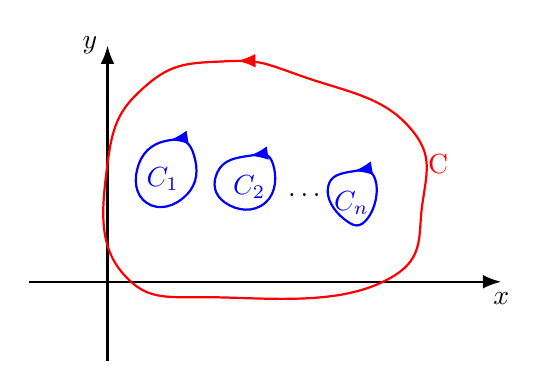
\begin{tikzpicture}[
    >=Latex, % Set default arrow tip style
    axis/.style={->, thick}, % Style for axes
    blob/.style={thick},     % Base style for blob borders
    % Style for placing a CCW arrow on a path
   midarrow/.style={
        decoration={markings, mark=at position 0.5 with {\arrow{Latex[length=2mm]}}},
        postaction={decorate}
    },
    midarrowL/.style={
        decoration={markings, mark=at position 0.2 with {\arrowreversed{Latex}}},
        postaction={decorate}
    }
]

    % Axes
    \draw[axis] (-1, 0) -- (5, 0) node[below] {$x$};
    \draw[axis] (0, -1) -- (0, 3) node[left] {$y$};

    % Define coordinates for outer blob C/Cn (adjust as needed)
    \def\coordsOuter{
        (0.2, 0.1) % Bottom left
        (0.0, 1.5) % Mid left
        (0.5, 2.5) % Top left
        (1.5, 2.8) % Top middle
        (2.5, 2.6) % Top right
        (3.8, 2.0) % Mid right
        (4.0, 1.0) % Lower right
        (3.5, 0.0) % Bottom right
        (1.5, -0.2)% Bottom middle
    }
    % Define coordinates for inner blobs (adjust as needed)
    \def\coordsC1{ (0.5, 1.0) (0.4, 1.5) (0.8, 1.8) (1.1, 1.6) (1.0, 1.1) }
    \def\coordsC2{ (1.5, 1.0) (1.4, 1.4) (1.8, 1.6) (2.1, 1.5) (2.0, 1.0) }
    \def\coordsCn{ (3.0, 0.8) (2.8, 1.2) (3.1, 1.4) (3.4, 1.3) (3.3, 0.8) }

    % Draw Outer Red Blob (C/Cn) with CCW Arrow
    \draw[blob, red, midarrowL] % Arrow on left side
        plot [smooth cycle, tension=0.8] coordinates {\coordsOuter};
   % \node[red] at (1.5, 3.0) {$C_n$}; % Label Cn at top
    \node[red] at (4.2, 1.5) {C};   % Label C at right

    % Draw Inner Blue Blobs with CW Arrows
    % C1
    \draw[blob, blue, midarrowL] % Arrow on left side
        plot [smooth cycle, tension=0.9] coordinates {(0.5, 1.0) (0.4, 1.5) (0.8, 1.8) (1.1, 1.6) (1.0, 1.1)};
    \node[blue] at (0.7, 1.3) {$C_1$}; % Label C1

    % C2
    \draw[blob, blue,midarrowL] % Arrow on left side
        plot [smooth cycle, tension=0.9] coordinates {\coordsC2};
    \node[blue] at (1.8, 1.2) {$C_2$}; % Label C2

    % Cn
    \draw[blob, blue, midarrowL] % Arrow on left side
        plot [smooth cycle, tension=0.9] coordinates {\coordsCn};
    \node[blue] at (3.1, 1.0) {$C_n$}; % Label Cn

    % Ellipsis between C2 and Cn
    \node at (2.5, 1.1) {$\dots$};

\end{tikzpicture}
\end{document}